% Exam only: four unmarked choices per question.
\noindent\begin{minipage}{\linewidth}
\small
\textbf{Câu 1.} Trong luồng sự kiện đơn hàng, phát biểu nào mô tả đúng trách nhiệm của các thành phần Kafka?
\begin{enumerate}[label=\textbf{\Alph*.},leftmargin=2em,itemsep=0pt,topsep=2pt]
\item Producer lưu mọi replica; broker cập nhật tồn kho; consumer quản lý metadata cluster.
\item Producer phân công consumer; broker chỉ lưu committed offset; consumer ghi mọi partition.
\item Producer gửi record; broker lưu và phục vụ dữ liệu; consumer đọc và thực hiện xử lý.
\item Producer gửi mọi record qua controller; consumer chỉ được đọc sau khi controller xử lý nghiệp vụ.
\end{enumerate}
\end{minipage}\par\addvspace{0.5em}

\noindent\begin{minipage}{\linewidth}
\small
\textbf{Câu 2.} Topic order-events có ba partition. Nhận định nào đúng về thứ tự và offset?
\begin{enumerate}[label=\textbf{\Alph*.},leftmargin=2em,itemsep=0pt,topsep=2pt]
\item Mỗi partition có thứ tự log riêng; offset 7 ở P0 và offset 7 ở P1 là hai vị trí khác nhau.
\item Kafka sắp mọi record trong cả topic theo một dãy offset duy nhất.
\item Record có timestamp nhỏ hơn luôn hoàn tất xử lý trước, bất kể partition.
\item Offset 7 của hai partition luôn chứa cùng một record vì đó là mã định danh toàn cục.
\end{enumerate}
\end{minipage}\par\addvspace{0.5em}

\noindent\begin{minipage}{\linewidth}
\small
\textbf{Câu 3.} Producer phân vùng theo key, giữ nguyên số partition, cách serialize key và thuật toán phân vùng. Các sự kiện cùng key o1001 sẽ có đặc điểm nào?
\begin{enumerate}[label=\textbf{\Alph*.},leftmargin=2em,itemsep=0pt,topsep=2pt]
\item Luôn được chia đều sang mọi partition để tăng tốc xử lý một đơn hàng.
\item Luôn ở partition 0 vì Kafka chỉ dùng key để lọc dữ liệu khi đọc.
\item Tạo một partition mới cho từng sự kiện có cùng key.
\item Được đưa vào cùng một partition theo chiến lược phân vùng đã nêu.
\end{enumerate}
\end{minipage}\par\addvspace{0.5em}

\noindent\begin{minipage}{\linewidth}
\small
\textbf{Câu 4.} Với Java producer mặc định ở mốc Kafka 4.1, nên giải thích thế nào khi một batch nhỏ không có key phân bố không đều giữa các partition?
\begin{enumerate}[label=\textbf{\Alph*.},leftmargin=2em,itemsep=0pt,topsep=2pt]
\item Kafka chắc chắn bị lỗi vì mọi ba record phải đi lần lượt qua P0, P1 và P2.
\item Producer có cơ chế sticky gắn với batching; không nên giả định round robin cho từng record.
\item Record không có key luôn được ghi đồng thời vào mọi partition của topic.
\item Consumer group quyết định partition của record ngay trước mỗi lần producer gửi.
\end{enumerate}
\end{minipage}\par\addvspace{0.5em}

\noindent\begin{minipage}{\linewidth}
\small
\textbf{Câu 5.} Một topic có 3 partition và replication factor bằng 3. Cách đếm nào đúng?
\begin{enumerate}[label=\textbf{\Alph*.},leftmargin=2em,itemsep=0pt,topsep=2pt]
\item Có 9 partition logic và 3 replica tổng cộng.
\item Có 3 partition logic và 12 replica vì leader không được tính vào replication factor.
\item Có 3 partition logic và 9 replica tổng cộng, trong đó có 3 leader.
\item Có 1 partition logic và 3 leader cùng nhận ghi cho partition đó.
\end{enumerate}
\end{minipage}\par\addvspace{0.5em}

\noindent\begin{minipage}{\linewidth}
\small
\textbf{Câu 6.} Giả sử ELR không bật, replication factor 3, ISR hiện có 3 replica, min.insync.replicas=2 và producer dùng acks=all. Phát biểu nào đúng?
\begin{enumerate}[label=\textbf{\Alph*.},leftmargin=2em,itemsep=0pt,topsep=2pt]
\item Chỉ cần leader ghi xong; acks=all bỏ qua follower khi min.insync.replicas nhỏ hơn 3.
\item Ngưỡng 2 kiểm tra ISR tối thiểu; acks=all chờ ISR hiện tại, không chỉ hai replica bất kỳ.
\item Lần ghi chỉ thành công sau khi mọi consumer group commit offset của record.
\item min.insync.replicas=2 làm Kafka giảm replication factor của topic xuống 2.
\end{enumerate}
\end{minipage}\par\addvspace{0.5em}

\Needspace{16\baselineskip}
\section*{Vận dụng: phân tích tình huống}
\noindent\begin{minipage}{\linewidth}
\small
\textbf{Câu 7.} Nhóm quan sát lag theo partition như trong sơ đồ và cần giữ thứ tự cho key có lưu lượng lớn.
\par\smallskip
\noindent\makebox[\linewidth][c]{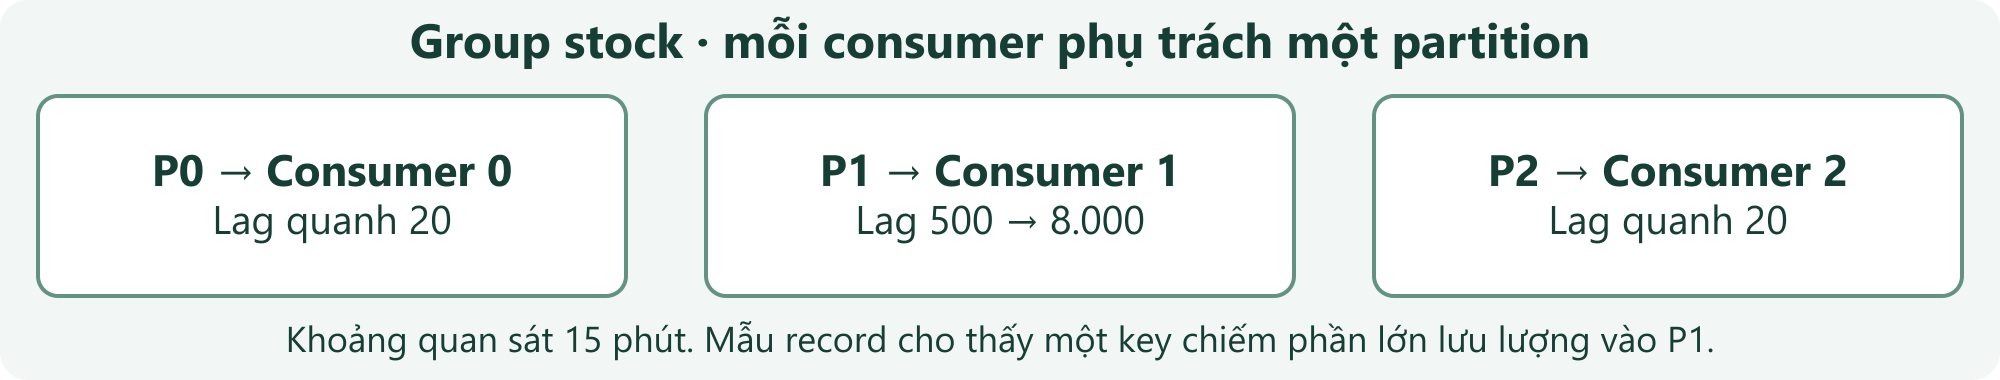
\includegraphics[width=0.96\linewidth]{Figures/case-7.png}}\par\smallskip
Bước xử lý đầu tiên hợp lý nhất là gì?
\begin{enumerate}[label=\textbf{\Alph*.},leftmargin=2em,itemsep=0pt,topsep=2pt]
\item Thêm consumer thứ tư để hai consumer cùng sở hữu P1 trong group hiện tại.
\item Tăng replication factor để follower chia đôi phần việc đọc P1 của group.
\item Đo thời gian xử lý và kiểm tra hệ thống đích của consumer P1; xem lại tải của key nóng trước khi đổi cách phân vùng.
\item Đổi toàn bộ key sang giá trị ngẫu nhiên để dàn tải, rồi giữ nguyên giả định thứ tự theo key.
\end{enumerate}
\end{minipage}\par\addvspace{0.5em}

\noindent\begin{minipage}{\linewidth}
\small
\textbf{Câu 8.} Nhóm đang thiết kế consumer group cho hai pipeline có yêu cầu như trong sơ đồ.
\par\smallskip
\noindent\makebox[\linewidth][c]{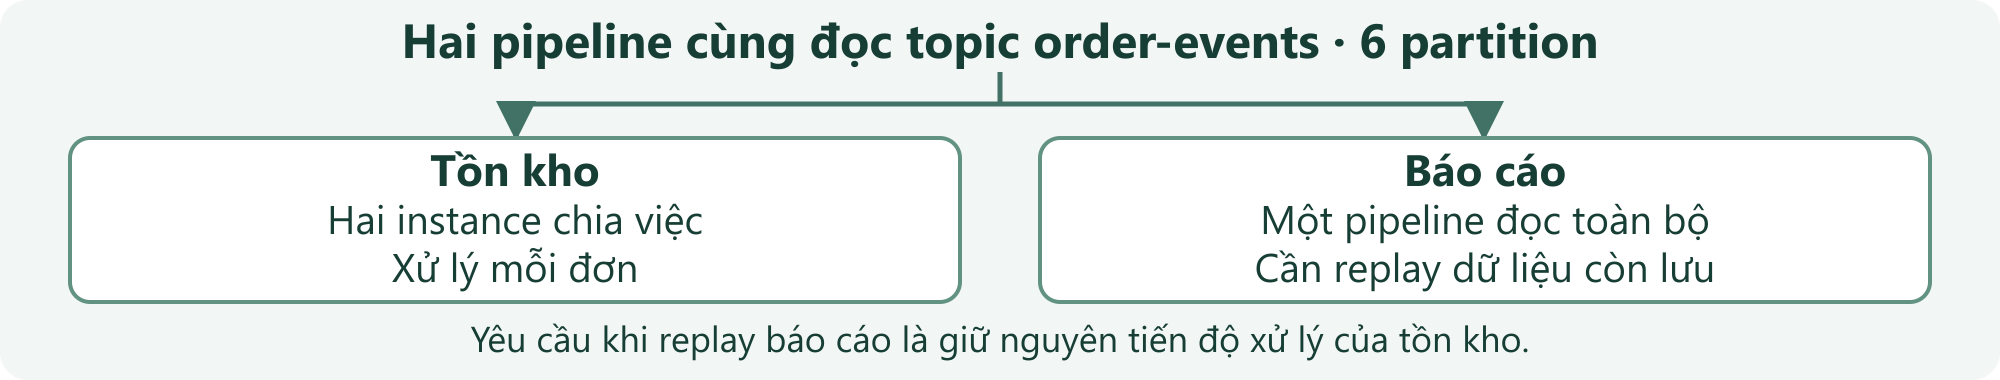
\includegraphics[width=0.96\linewidth]{Figures/case-8.png}}\par\smallskip
Kiến trúc nào đáp ứng đồng thời việc chia tải và đọc độc lập?
\begin{enumerate}[label=\textbf{\Alph*.},leftmargin=2em,itemsep=0pt,topsep=2pt]
\item Dùng hai instance cùng group \texttt{stock}; báo cáo dùng group khác và chọn vị trí replay riêng của báo cáo.
\item Đưa cả ba instance vào group \texttt{stock}, rồi cho báo cáo chạy từ đầu khi cần.
\item Cho từng instance tồn kho một group riêng; dựa vào replication factor để tránh xử lý trùng giữa chúng.
\item Tăng số replica và giữ một group chung; mỗi follower tự lưu offset riêng cho từng pipeline.
\end{enumerate}
\end{minipage}\par\addvspace{0.5em}

\noindent\begin{minipage}{\linewidth}
\small
\textbf{Câu 9.} Producer gặp lỗi khi ghi P2. Sơ đồ thể hiện cấu hình topic và trạng thái từng replica.
\par\smallskip
\noindent\makebox[\linewidth][c]{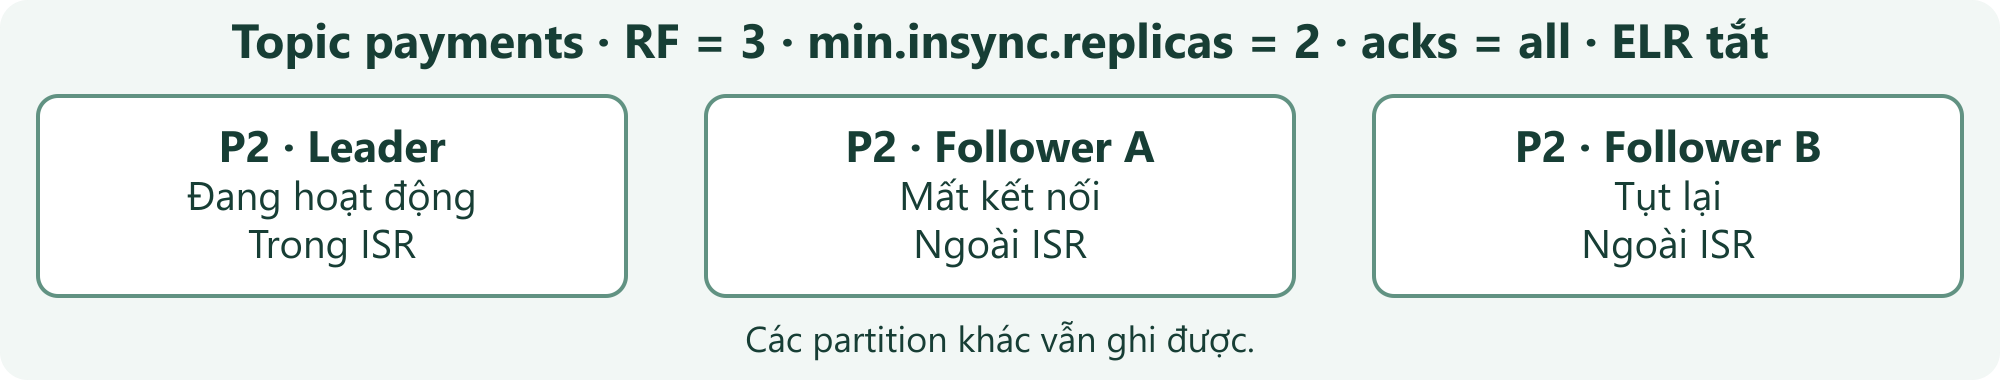
\includegraphics[width=0.96\linewidth]{Figures/case-9.png}}\par\smallskip
Kết luận và hướng khôi phục nào phù hợp nếu phải giữ chính sách xác nhận hiện tại?
\begin{enumerate}[label=\textbf{\Alph*.},leftmargin=2em,itemsep=0pt,topsep=2pt]
\item P2 vẫn ghi thành công vì replication factor trên cấu hình vẫn là 3; chỉ cần tăng timeout producer.
\item P2 không đáp ứng ngưỡng ISR; khôi phục ít nhất một follower và xác nhận ISR trở lại từ 2 thành viên trước khi kỳ vọng lần ghi thành công.
\item Cần thêm consumer cho P2 để consumer gửi xác nhận thay follower.
\item Hạ \texttt{min.insync.replicas} xuống 1; như vậy vẫn giữ nguyên yêu cầu có ít nhất hai replica theo kịp.
\end{enumerate}
\end{minipage}\par\addvspace{0.5em}

\noindent\begin{minipage}{\linewidth}
\small
\textbf{Câu 10.} Consumer tồn kho gặp sự cố tại thời điểm trong sơ đồ.
\par\smallskip
\noindent\makebox[\linewidth][c]{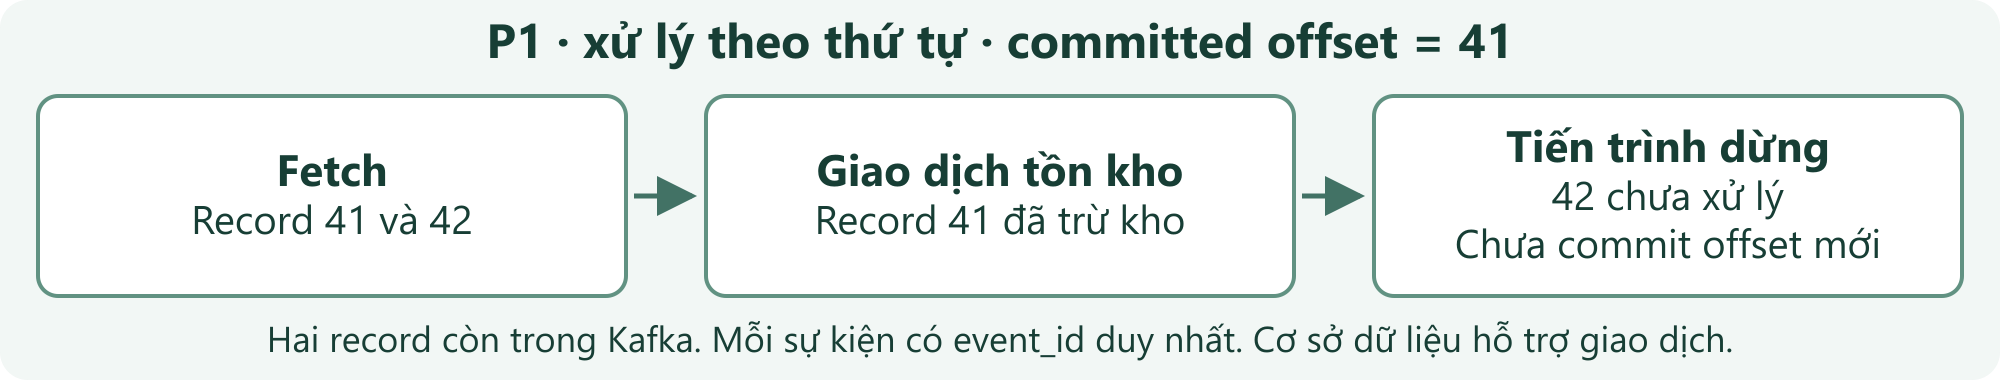
\includegraphics[width=0.96\linewidth]{Figures/case-10.png}}\par\smallskip
Thiết kế nào cho phép phục hồi mà không bỏ sót 42 hoặc trừ kho hai lần cho 41?
\begin{enumerate}[label=\textbf{\Alph*.},leftmargin=2em,itemsep=0pt,topsep=2pt]
\item Khi khởi động lại, luôn seek đến offset 43 vì cả hai record đã được fetch trước khi lỗi.
\item Bật producer idempotence rồi tiếp tục trừ kho vô điều kiện cho mọi record được đọc lại.
\item Commit offset 43 ngay sau khi poll; nếu trừ kho thất bại thì chờ Kafka tự phát lại.
\item Đọc lại từ mốc 41, ghi dấu \texttt{event\_id} và cập nhật tồn kho trong cùng giao dịch khi xử lý mới; bỏ qua tác động đã ghi nhận rồi commit đến vị trí tiếp theo sau khi xử lý xong.
\end{enumerate}
\end{minipage}\par\addvspace{0.5em}
